\vspace*{-1cm}

\nombreCapituloCabecera{RH}{Diseño del laboratorio}

\section{Diseño del laboratorio}
\label{sec:diseno_del_laboratorio}

\begin{figure}[H]
    \centering
    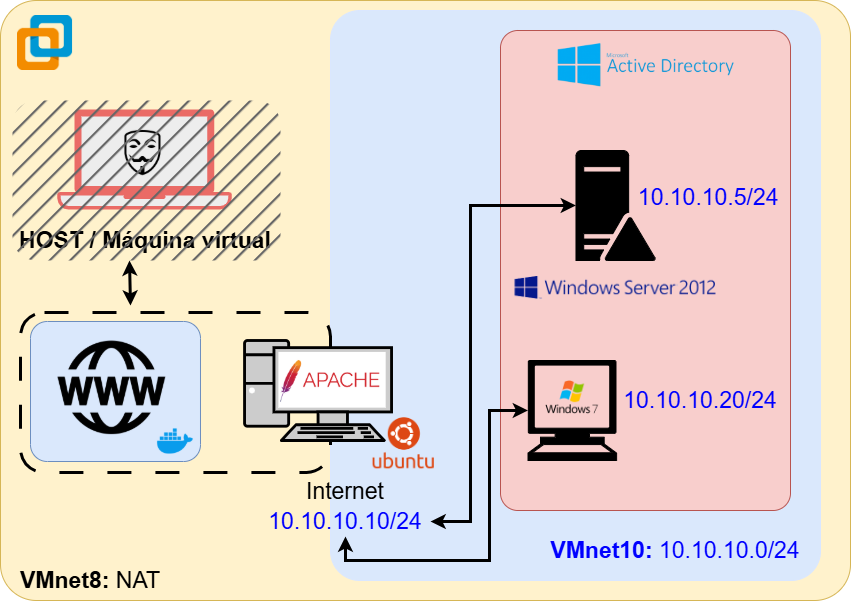
\includegraphics[width=1\textwidth]{Imagenes/Diagrama-completo.png}

    \vspace{0.2cm}
    \captionazul{Diagrama completo de la infraestructura del laboratorio, mostrando los sistemas, servicios, segmentos de red y relaciones entre componentes.}

    \label{fig:diagrama_completo_laboratorio}
\end{figure}


El diseño del laboratorio constituye uno de los elementos fundamentales del proyecto, ya que determina la forma en la que se desarrollarán los distintos escenarios de ataque y condiciona la capacidad del entorno para reproducir situaciones reales. El objetivo principal ha sido construir una infraestructura que simule una pequeña organización con servicios expuestos a Internet y una red interna basada en tecnologías Microsoft, permitiendo encadenar diferentes fases de una intrusión de forma controlada.

Para ello se ha optado por una arquitectura compuesta por varios sistemas virtualizados que representan distintos activos de una empresa. Esta aproximación permite separar los diferentes servicios, facilitar la gestión del entorno y reproducir de forma más realista las técnicas utilizadas habitualmente durante ejercicios de Red Team y pruebas de penetración.

La infraestructura resultante combina sistemas Linux y Windows, servicios web basados en PHP con docker y apache, Active Directory y estaciones de trabajo corporativas, proporcionando múltiples superficies de ataque y permitiendo la ejecución de escenarios que abarcan desde la explotación inicial de una vulnerabilidad web hasta el compromiso
completo de una infraestructura interna.

% ==========================================================
\subsection{Arquitectura general}
% ==========================================================

La arquitectura general del laboratorio ha sido diseñada siguiendo una estructura escalonada que obliga al atacante a progresar a través de distintas fases de compromiso. De esta forma, el acceso a los sistemas internos no es directo, sino que requiere explotar vulnerabilidades, obtener credenciales y realizar movimientos laterales similares a los que se producen en ataques reales.

El entorno está compuesto por tres máquinas virtuales principales que  onstituyen la infraestructura vulnerable:

\begin{itemize}
    \item Un servidor Ubuntu Server 22.04 encargado de alojar la aplicación web
          vulnerable.
    \item Un controlador de dominio Windows Server 2012 denominado \texttt{DC01}.
    \item Una estación de trabajo Windows 7 denominada \texttt{DEV01}.
\end{itemize}

Estas máquinas representan los principales elementos que pueden encontrarse en una pequeña o mediana empresa y permiten implementar escenarios de ataque progresivos que combinan vulnerabilidades web con técnicas de post-explotación sobre entornos Windows.

La máquina atacante no forma parte del laboratorio vulnerable como tal. Dependiendo del escenario de despliegue, el usuario puede utilizar directamente el sistema anfitrión como plataforma de ataque si dispone de una distribución especializada como Kali Linux o Parrot OS, o bien desplegar una máquina virtual adicional dedicada a tareas ofensivas.

El diseño busca mantener un equilibrio entre realismo y simplicidad. Por un lado, incorpora suficientes componentes para permitir escenarios complejos de explotación; por otro, evita una infraestructura excesivamente grande que dificultaría su despliegue en equipos domésticos o académicos.

% IMAGEN RECOMENDADA
% Diagrama general de la arquitectura mostrando:
% Host -> Ubuntu Web -> DC01 -> DEV01

% ==========================================================
\subsubsection{Arquitectura física}
% ==========================================================

Desde una perspectiva física, toda la infraestructura se ejecuta sobre un único equipo anfitrión utilizando VMware Workstation como plataforma de virtualización. Cada sistema se encuentra encapsulado en una máquina virtual independiente, permitiendo asignar recursos específicos a cada componente y facilitando la gestión del laboratorio.

La utilización de máquinas virtuales aporta varias ventajas relevantes para este proyecto. En primer lugar, permite mantener completamente aislado el entorno vulnerable respecto al sistema anfitrión. En segundo lugar, facilita la creación de instantáneas que permiten restaurar rápidamente el estado del laboratorio después de una explotación o durante las tareas de validación. Finalmente, mejora la portabilidad del proyecto, ya que las máquinas pueden trasladarse entre distintos equipos sin necesidad de repetir todo el proceso de instalación.

Cada máquina virtual dispone de una función específica dentro de la infraestructura. El servidor Ubuntu aloja los servicios expuestos al exterior y constituye el principal punto de entrada para el atacante. El controlador de dominio centraliza la autenticación y la gestión de usuarios dentro de la red corporativa, mientras que la estación de trabajo representa un equipo interno susceptible de ser comprometido mediante técnicas de movimiento lateral.

Esta distribución permite reproducir de forma realista la separación habitual entre sistemas expuestos y sistemas internos presente en muchas organizaciones.

Las Figuras~\ref{fig:configuracion_maquinas_virtuales} y~\ref{fig:configuracion_vm} recogen la configuración física asignada a las máquinas virtuales del laboratorio. La primera resume los parámetros principales de cada sistema, incluyendo recursos hardware, direccionamiento de red y rol dentro de la infraestructura. La segunda muestra dicha configuración desde VMware Workstation, permitiendo comprobar la asignación real de memoria, CPU, disco e interfaces de red utilizadas durante el despliegue.

\begin{figure}[H]
\centering

\begin{minipage}[t]{0.33\textwidth}
\begin{tcolorbox}[
    colback=orange!5,
    colframe=orange!70!black,
    title=\small\textbf{🧱 Ubuntu Server 22.04},
    fonttitle=\bfseries,
    boxrule=0.5pt]

\footnotesize
\textbf{Nombre}\\
\texttt{ubuntu-server-TFM}

\vspace{0.2cm}

\textbf{ISO}\\
ubuntu-22.04.4-live-server-amd64.iso

\vspace{0.2cm}

\textbf{CPU}: 2 cores

\textbf{RAM}: 3 GB

\textbf{Disco}: 40 GB (thin)

\textbf{VMnet8}: DHCP

\textbf{VMnet10}: 10.10.10.10/24

\textbf{Rol}\\
Servidor web vulnerable

\end{tcolorbox}
\end{minipage}
\hfill
\begin{minipage}[t]{0.30\textwidth}
\begin{tcolorbox}[
    colback=cyan!5,
    colframe=cyan!70!black,
    title=\small\textbf{💻 DEV01},
    fonttitle=\bfseries,
    boxrule=0.5pt]

\footnotesize
\textbf{Nombre}\\
DEV01

\vspace{0.2cm}

\textbf{ISO}\\
Windows 7 Professional

\vspace{0.2cm}

\textbf{CPU}: 2 cores

\textbf{RAM}: 3 GB

\textbf{Disco}: 40 GB (thin)

\textbf{IP}: 10.10.10.20/24

\textbf{Rol}\\
Estación de trabajo

\end{tcolorbox}
\end{minipage}
\hfill
\begin{minipage}[t]{0.30\textwidth}
\begin{tcolorbox}[
    colback=blue!5,
    colframe=blue!70!black,
    title=\small\textbf{🪟 DC01},
    fonttitle=\bfseries,
    boxrule=0.5pt]

\footnotesize
\textbf{Nombre}\\
DC01

\vspace{0.2cm}

\textbf{ISO}\\
Windows Server 2012

\vspace{0.2cm}

\textbf{CPU}: 2 cores

\textbf{RAM}: 4 GB

\textbf{Disco}: 60 GB (thin)

\textbf{IP}: 10.10.10.5/24

\textbf{Dominio}: corp.local

\textbf{Rol}\\
Controlador de dominio

\end{tcolorbox}
\end{minipage}

\vspace{0.3cm}

\captionazul{Configuración de las máquinas virtuales que componen la infraestructura del laboratorio.}
\label{fig:configuracion_maquinas_virtuales}

\end{figure}


\begin{figure}[H]
    \centering
    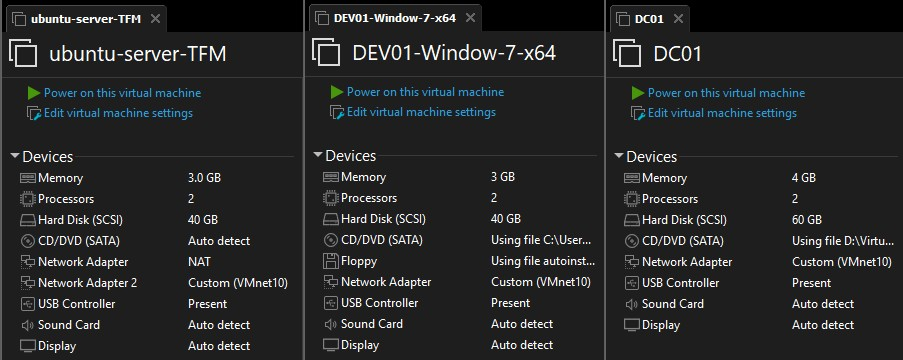
\includegraphics[width=1\textwidth]{Imagenes/configuracion-VM-vmware.jpg}

    \vspace{0.2cm}
    \captionazul{Configuración de las máquinas virtuales en VMware Workstation, mostrando la asignación de recursos hardware para cada sistema.}
    \label{fig:configuracion_vm}
\end{figure}



% ==========================================================
\subsubsection{Optimización de recursos}
% ==========================================================

Uno de los objetivos perseguidos durante el diseño del laboratorio ha sido garantizar que la infraestructura pudiera ejecutarse sobre equipos domésticos o académicos sin requerir una gran capacidad hardware.

Aunque VMware Workstation propone configuraciones de memoria superiores para los sistemas operativos utilizados, se realizaron diversas pruebas de ajuste con el objetivo de determinar los recursos mínimos necesarios para mantener un funcionamiento estable del entorno.

Tras varias iteraciones se comprobó que era posible reducir significativamente la memoria asignada a las máquinas virtuales sin afectar al correcto desarrollo de los escenarios de ataque ni al funcionamiento de los servicios desplegados. La Tabla~\ref{tab:optimizacion_memoria} resume la configuración mínima validada durante las pruebas realizadas.

\vspace{0.5cm}
\renewcommand{\arraystretch}{1.4}

\begin{table}[H]
    \centering
    \captionazul{Configuración mínima de memoria validada para las máquinas virtuales}

    \begin{tabular}{|C{6cm}|C{3cm}|}
        \hline
        \rowcolor{blue!10}
        \textbf{Sistema} & \textbf{Memoria RAM}  \\
        \hline
        Ubuntu Server 22.04 & 1.5 GB  \\
        \hline
        DC01 (Windows Server 2012) & 1.2 GB  \\
        \hline
        DEV01 (Windows 7) & 1.5 GB  \\
        \hline
    \end{tabular}

    \renewcommand{\arraystretch}{1}
    \label{tab:optimizacion_memoria}
\end{table}

Estas pruebas permitieron reducir el consumo total de memoria de la infraestructura hasta aproximadamente 4.2 GB, lo que facilita la ejecución simultánea de todas las máquinas virtuales incluso en equipos con recursos limitados.

La reducción de recursos no afecta al comportamiento del laboratorio ni a la reproducibilidad de las cadenas de ataque implementadas, manteniendo el equilibrio entre realismo y accesibilidad que se persigue en este proyecto.

\begin{figure}[H]
    \centering

    \begin{subfigure}{1\textwidth}
        \centering
        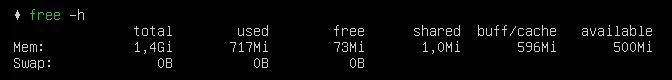
\includegraphics[width=\textwidth]{Imagenes/memoria-optimizada-WEB-SERVER.png}
        \subcaption{\textcolor{blueColor}Servidor web Ubuntu}
    \end{subfigure}

    \vspace{0.5cm}

    \begin{subfigure}{1\textwidth}
        \centering
        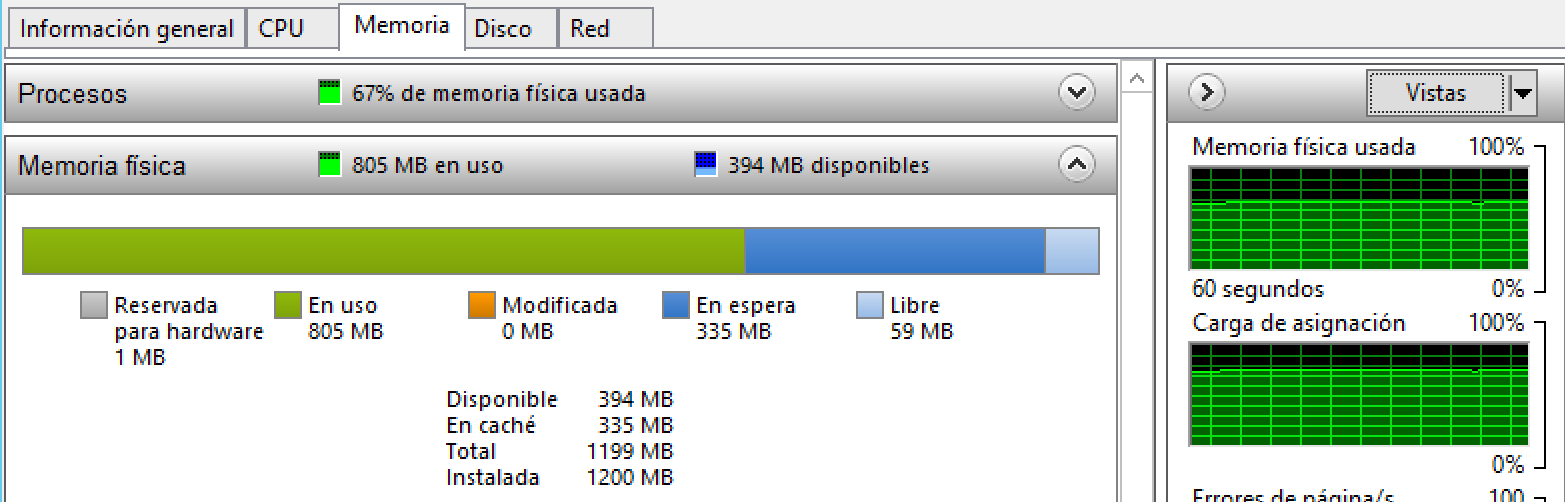
\includegraphics[width=\textwidth]{Imagenes/memoria-optimizada-DC01.png}
        \subcaption{\textcolor{blueColor}Controlador de dominio DC01}
    \end{subfigure}

    \vspace{0.5cm}

    \begin{subfigure}{1\textwidth}
        \centering
        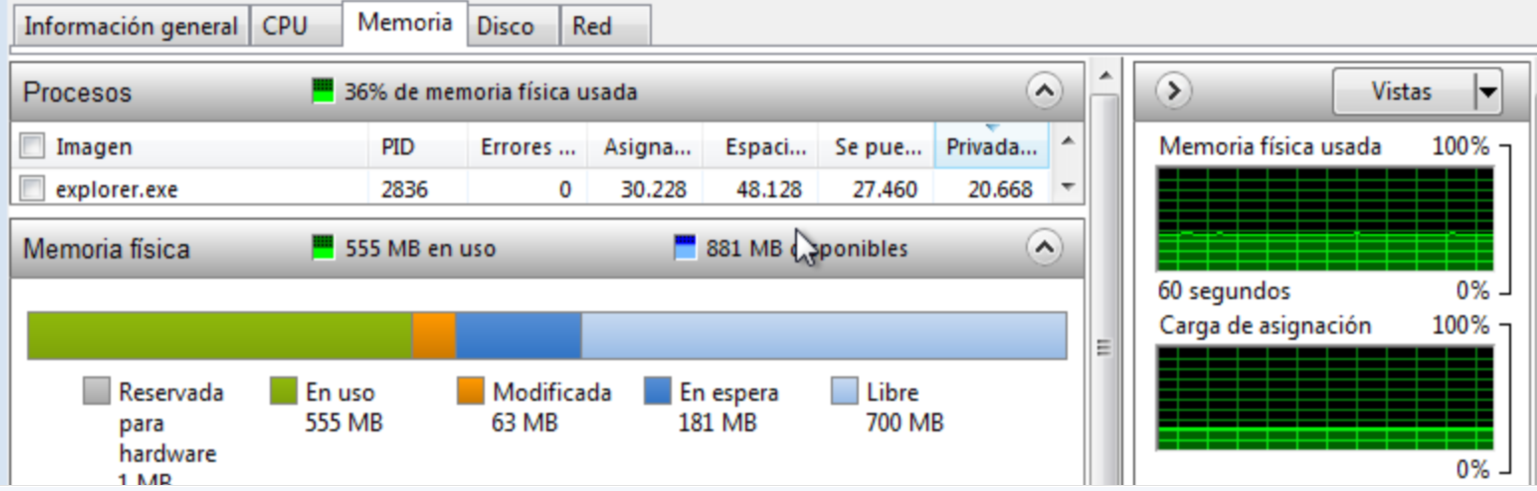
\includegraphics[width=\textwidth]{Imagenes/memoria-optimizada-Dev01.png}
        \subcaption{\textcolor{blueColor}Estación de trabajo DEV01}
    \end{subfigure}

    \vspace{0.5cm}
    \captionazul{Optimización de la memoria RAM asignada a las máquinas virtuales del laboratorio.}
    \label{fig:optimizacion_memoria_lab}
\end{figure}


Las capturas mostradas en la Figura~\ref{fig:optimizacion_memoria_lab} evidencian el consumo real de memoria de las tres máquinas virtuales tras completar el proceso de optimización. Los resultados obtenidos demuestran que tanto Windows Server 2012 como Windows 7 y Ubuntu Server mantienen una cantidad suficiente de memoria disponible para ejecutar los servicios necesarios del laboratorio.

En el caso del controlador de dominio DC01, con únicamente 1.2 GB de memoria asignada, el sistema conserva aproximadamente 400 MB libres una vez iniciados Active Directory y el servicio DNS. De forma similar, la estación de trabajo DEV01 dispone de cerca de 900 MB disponibles con una asignación total de 1.5 GB, mientras que el servidor Ubuntu mantiene alrededor de 500 MB de memoria disponible tras el despliegue de Docker y del portal vulnerable.

Estos resultados confirman que las recomendaciones de memoria propuestas por VMware Workstation pueden reducirse considerablemente para este escenario concreto sin comprometer la estabilidad de los servicios ni la reproducibilidad de las cadenas de ataque implementadas.

La optimización realizada permite ejecutar simultáneamente toda la infraestructura utilizando aproximadamente 4.2 GB de memoria RAM, facilitando el despliegue del laboratorio en equipos domésticos o académicos con recursos limitados y contribuyendo a uno de los objetivos principales del proyecto: proporcionar un entorno de entrenamiento accesible sin renunciar al realismo del escenario.

Los valores de memoria finalmente adoptados fueron utilizados durante todas las pruebas de validación y explotación descritas en el Capítulo~\ref{sec:explotacion_del_laboratorio}, verificándose que no introducen limitaciones apreciables en el desarrollo de los distintos escenarios ofensivos implementados.

% ==========================================================
\subsubsection{Arquitectura lógica}
% ==========================================================

A nivel lógico, la infraestructura se divide en dos niveles de acceso que representan las distintas fases de compromiso que debe superar un atacante.

El primer nivel está formado por los servicios accesibles inicialmente desde la red del atacante. Dentro de este nivel se encuentra el portal web vulnerable desplegado sobre Ubuntu Server sobre un contenedor Docker, que actúa como punto de entrada principal al laboratorio.

El segundo nivel corresponde a la infraestructura interna basada en Active Directory. Esta red contiene los sistemas corporativos que no son accesibles directamente desde el exterior y que requieren un compromiso previo para poder ser alcanzados. El acceso a estos sistemas obliga al atacante a obtener credenciales válidas, realizar tarea  de enumeración y aprovechar relaciones de confianza existentes dentro de la infraestructura.

La separación lógica entre estos niveles no solo mejora el realismo del laboratorio, sino que también permite analizar con mayor claridad las distintas etapas de un ataque y estudiar cómo pequeños fallos de seguridad pueden combinarse para producir un compromiso completo de la organización.

\begin{figure}[H]
    \centering
    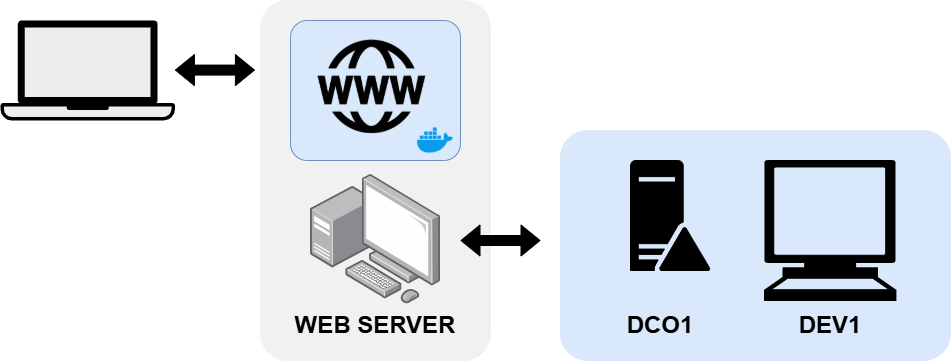
\includegraphics[width=0.8\textwidth]{Imagenes/activos-ataque.png}

    \vspace{0.2cm}
    \captionazul{Diagrama de la arquitectura lógica del laboratorio, mostrando los niveles de acceso y las relaciones entre los distintos sistemas.}
    \label{fig:arquitectura_logica}
\end{figure}



% ==========================================================
\subsubsection{Segmentación de red}
% ==========================================================

La segmentación de red constituye uno de los mecanismos principales utilizados para aumentar el realismo del laboratorio y controlar las comunicaciones entre los distintos sistemas. En lugar de conectar todas las máquinas a una misma red virtual, se han definido diferentes segmentos que permiten simular la separación habitual existente entre servicios públicos e infraestructura interna. Esta división obliga al atacante a utilizar técnicas de pivoting y movimiento lateral para progresar dentro del entorno.

El servidor Ubuntu actúa como punto intermedio entre la red utilizada por el atacante y la infraestructura interna. Una vez comprometido este sistema, es posible acceder a recursos que inicialmente no eran visibles, reproduciendo así escenarios habituales de intrusión corporativa.

Además de mejorar el realismo de los escenarios de ataque, esta segmentación permite controlar con precisión qué servicios son accesibles desde cada zona de la infraestructura y facilita la implementación de ejercicios relacionados con enumeración de red, descubrimiento de servicios internos y explotación de relaciones de confianza.

La estructura de red adoptada proporciona un equilibrio adecuado entre complejidad y facilidad de despliegue, permitiendo reproducir técnicas avanzadas sin incrementar excesivamente los requisitos hardware del laboratorio.

\begin{figure}[H]
    \centering
    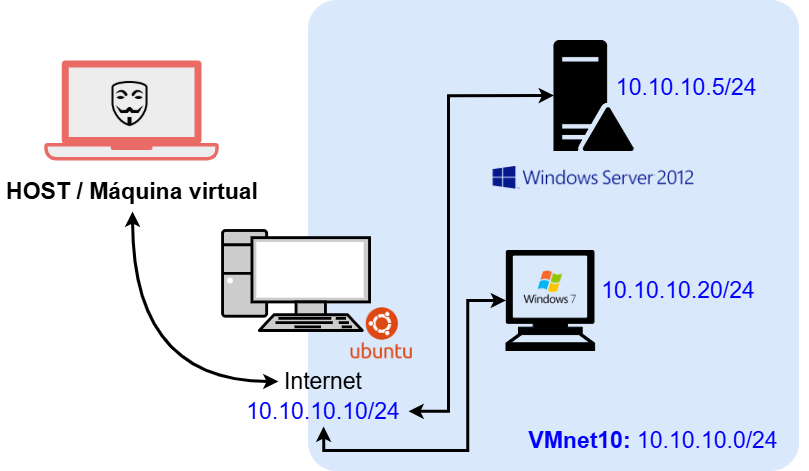
\includegraphics[width=0.85\textwidth]{Imagenes/esquema-detallado-redes-VMware-interfaces.png}

    \vspace{0.2cm}
    \captionazul{Esquema detallado de la segmentación de red y configuración de interfaces en VMware Workstation.}

    \label{fig:esquema_redes}
\end{figure}

\begin{figure}[H]
    \centering
    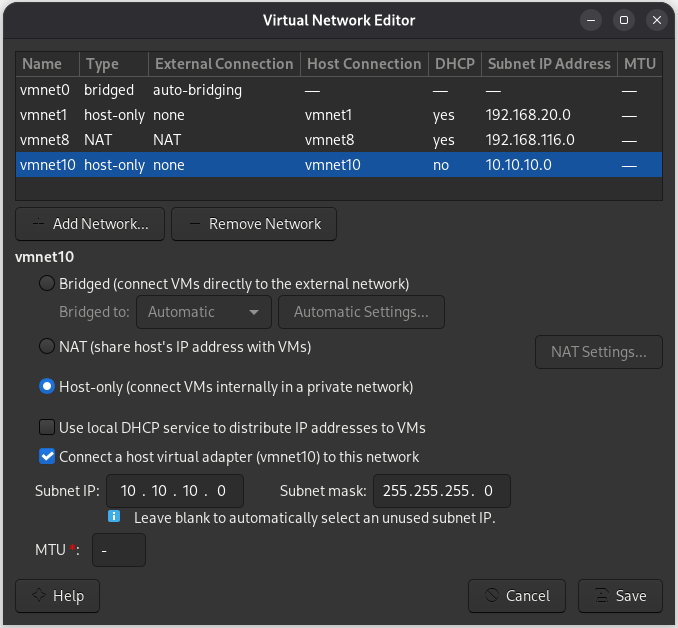
\includegraphics[width=0.9\textwidth]{Imagenes/segmentacion-red-vmware.png}

    \vspace{0.2cm}
    \captionazul{Configuracion de la red en VMware}

    \label{fig:segmentacion_red-vmware}
\end{figure}


% ==========================================================
\subsection{Diseño del servidor vulnerable}
% ==========================================================

El servidor vulnerable constituye el elemento central del laboratorio y representa el principal punto de entrada para los escenarios de ataque implementados. Su diseño persigue reproducir las características de un servidor corporativo real que aloja una aplicación web accesible por los usuarios de la organización.

Para su implementación se ha seleccionado Ubuntu Server 22.04 como sistema operativo base debido a su estabilidad, amplia documentación y elevada adopción dentro de entornos empresariales. Sobre este sistema se despliegan los distintos servicios necesarios para ejecutar la aplicación vulnerable y proporcionar funcionalidades similares a las que podrían encontrarse en una pequeña empresa.

El servidor no se limita únicamente a alojar una aplicación web vulnerable, sino que también incorpora configuraciones inseguras, credenciales expuestas y distintos elementos destinados a facilitar la construcción de cadenas de ataque complejas. De esta forma, una vulnerabilidad inicial puede convertirse en el punto de partida para comprometer otros sistemas de la infraestructura.

El diseño del servidor se ha realizado intentando mantener un equilibrio entre realismo y valor didáctico. Las vulnerabilidades introducidas son representativas de problemas observados frecuentemente en entornos reales, pero han sido adaptadas para garantizar que puedan ser explotadas de forma controlada dentro del laboratorio.

% IMAGEN RECOMENDADA
% Vista general del servidor Ubuntu y servicios desplegados.

% ==========================================================
\subsubsection{Stack tecnológico}
% ==========================================================

La aplicación vulnerable se apoya sobre una pila tecnológica basada en componentes ampliamente utilizados en entornos reales. La selección de estas tecnologías permite que los escenarios desarrollados resulten representativos de situaciones que pueden encontrarse habitualmente durante auditorías de seguridad o ejercicios de Red Team.

El sistema operativo utilizado es Ubuntu Server 22.04. Sobre él se despliegan los servicios web necesarios para alojar la aplicación vulnerable y la base de datos asociada.

Para simplificar el despliegue y mejorar la reproducibilidad del entorno se ha optado por utilizar Docker y Docker Compose. Esta aproximación permite encapsular los distintos componentes de la aplicación y garantizar que el comportamiento del laboratorio sea consistente independientemente del equipo anfitrión utilizado.

La lógica de negocio del portal se ha desarrollado utilizando PHP, mientras que el almacenamiento de la información se realiza mediante MySQL. Finalmente, Apache HTTP Server actúa como servidor web encargado de atender las peticiones realizadas por los usuarios.

\vspace{0.5cm}
\renewcommand{\arraystretch}{1.5}

\begin{table}[h]
    \centering
    \captionazul{Stack tecnológico utilizado en el servidor vulnerable}

    \setlength{\arrayrulewidth}{0.05mm}

    \begin{tabular}{|C{5cm}|C{8cm}|}
        \hline
        \rowcolor{blue!10}
        \textbf{Componente} & \textbf{Función}             \\
        \hline
        Ubuntu Server 22.04 & Sistema operativo base       \\
        \hline
        Docker              & Contenerización de servicios \\
        \hline
        Docker Compose      & Orquestación de contenedores \\
        \hline
        Apache HTTP Server  & Servidor web                 \\
        \hline
        PHP                 & Lógica de aplicación         \\
        \hline
        MySQL               & Base de datos                \\
        \hline
    \end{tabular}

    \renewcommand{\arraystretch}{1}
    \label{tab:stack_tecnologico}
\end{table}

\vspace{0.5cm}

% ==========================================================
\subsubsection{Portal web vulnerable}
% ==========================================================

Con el objetivo de evitar el uso de aplicaciones deliberadamente inseguras y aumentar el realismo del laboratorio, se desarrolló una aplicación web propia denominada \textit{Portal PYME}.

La aplicación simula un sistema de gestión utilizado por una pequeña organización y proporciona funcionalidades similares a las que pueden encontrarse en numerosos entornos empresariales. Entre ellas destacan la gestión de usuarios, la administración de clientes, el control de empleados y la gestión de incidencias mediante un sistema de tickets.

A diferencia de laboratorios clásicos como DVWA o Mutillidae, el portal desarrollado para este proyecto intenta presentar una apariencia más cercana a una aplicación corporativa real. Esto permite que las vulnerabilidades implementadas se integren de forma natural dentro del flujo de funcionamiento de la aplicación y facilita la construcción de escenarios de ataque más creíbles.

El portal constituye el principal punto de entrada al laboratorio y concentra la mayor parte de las vulnerabilidades utilizadas durante los distintos ejercicios de explotación.

% IMAGEN RECOMENDADA
% Captura de la página principal del Portal PYME.

% ==========================================================
\subsubsection{Vulnerabilidades implementadas}
% ==========================================================

Las vulnerabilidades incorporadas en el laboratorio han sido seleccionadas tomando como referencia las categorías definidas por OWASP Top 10, así como errores de configuración y malas prácticas frecuentemente observadas durante auditorías de seguridad reales.

El objetivo no consiste únicamente en demostrar la explotación aislada de cada vulnerabilidad, sino permitir la construcción de cadenas de ataque completas donde una debilidad inicial proporcione acceso a nuevos recursos, credenciales o sistemas internos.

Durante el diseño del laboratorio se ha buscado que las vulnerabilidades se encuentren integradas de forma natural dentro del funcionamiento de la aplicación, evitando mecanismos artificiales que reduzcan el realismo del entorno. De esta forma, el atacante debe realizar tareas de reconocimiento, enumeración y análisis antes de identificar los vectores de explotación disponibles.

Además de las vulnerabilidades presentes en la aplicación web, el laboratorio incorpora configuraciones inseguras y mecanismos de escalada de privilegios tanto en el entorno Linux como en la infraestructura Windows, permitiendo reproducir diferentes fases de una intrusión real.

\vspace{0.5cm}
\renewcommand{\arraystretch}{1.5}

\begin{table}[h]
    \centering
    \captionazul{Categorías de vulnerabilidades implementadas en el laboratorio}

    \setlength{\arrayrulewidth}{0.05mm}

    \begin{tabular}{|C{5cm}|C{8cm}|}
        \hline
        \rowcolor{blue!10}
        \textbf{Categoría}              & \textbf{Objetivo}                     \\
        \hline
        Vulnerabilidades web            & Obtener acceso inicial al entorno     \\
        \hline
        Exposición de credenciales      & Facilitar el acceso a otros sistemas  \\
        \hline
        Escalada de privilegios Linux   & Obtener control completo del servidor \\
        \hline
        Configuraciones inseguras       & Aumentar la superficie de ataque      \\
        \hline
        Movimiento lateral              & Acceder a la infraestructura interna  \\
        \hline
        Debilidades en Active Directory & Comprometer recursos corporativos     \\
        \hline
    \end{tabular}

    \renewcommand{\arraystretch}{1}
    \label{tab:vulnerabilidades_laboratorio}
\end{table}

\vspace{0.5cm}

% IMAGEN RECOMENDADA
% Tabla resumen OWASP Top 10 implementado
% o captura de funcionalidades vulnerables del Portal PYME.

% ==========================================================
\subsection{Diseño de la infraestructura Active Directory}
% ==========================================================

La incorporación de una infraestructura Active Directory permite ampliar significativamente las posibilidades del laboratorio y reproducir escenarios de ataque que van más allá de la explotación inicial de una aplicación web.

En numerosos incidentes de seguridad reales, el compromiso de un servidor expuesto constituye únicamente la primera fase de la intrusión. Una vez obtenido acceso inicial, los atacantes suelen intentar acceder a sistemas internos, obtener credenciales corporativas y comprometer servicios de autenticación centralizados.

Con el objetivo de reproducir este tipo de situaciones, se ha diseñado una infraestructura Windows compuesta por un controlador de dominio y una estación de trabajo integrada en el dominio. Ambos sistemas permiten desarrollar ejercicios de enumeración, movimiento lateral, abuso de credenciales y post-explotación.

La arquitectura propuesta mantiene un nivel de complejidad suficiente para simular un entorno empresarial realista sin incrementar excesivamente los requisitos hardware necesarios para su ejecución.

Los detalles completos relativos a la instalación y personalización de la infraestructura Active Directory se incluyen en el Anexo~\ref{anexo:implementacion_active_directory}: \textit{Implementación de Active Directory}, donde se documenta el proceso de promoción del controlador de dominio, la creación de usuarios y grupos, la configuración de políticas y la integración de los equipos del dominio.

% IMAGEN RECOMENDADA
% Diagrama simplificado de Active Directory.

% ==========================================================
\subsubsection{Controlador de dominio - DC01}
% ==========================================================

DC01 constituye el controlador de dominio principal del laboratorio y representa el núcleo de la infraestructura Windows desplegada.

Este sistema se encuentra basado en Windows Server 2012 y proporciona los servicios necesarios para gestionar la autenticación, autorización y administración centralizada de usuarios y equipos. Desde este servidor se gestionan las cuentas de usuario, los grupos de seguridad, las políticas de dominio y diversos servicios internos necesarios para el funcionamiento de la organización simulada.

La elección de Windows Server 2012 responde a su amplia presencia histórica en entornos corporativos y a la disponibilidad de numerosas técnicas de ataque documentadas que permiten desarrollar escenarios de explotación realistas.

Desde la perspectiva ofensiva, DC01 constituye uno de los objetivos principales del laboratorio, ya que su compromiso permite acceder a información sensible y obtener control sobre el resto de sistemas integrados en el dominio.

% IMAGEN RECOMENDADA
% Captura del Administrador del Servidor o Active Directory Users and Computers.

% ==========================================================
\subsubsection{Estación de trabajo - DEV01}
% ==========================================================

DEV01 representa una estación de trabajo corporativa integrada dentro del dominio gestionado por DC01.

Este sistema se encuentra basado en Windows 7 y simula el equipo utilizado por un empleado de la organización. Su presencia dentro del laboratorio permite reproducir escenarios habituales de movimiento lateral y acceso a recursos internos tras comprometer otros sistemas de la infraestructura.

La estación de trabajo almacena información corporativa, credenciales y configuraciones que pueden resultar de interés para un atacante durante las fases posteriores de una intrusión.

La existencia de un equipo cliente integrado en Active Directory permite además evaluar las relaciones de confianza existentes dentro del dominio y reproducir técnicas de post-explotación ampliamente utilizadas en entornos Windows.

% IMAGEN RECOMENDADA
% Escritorio de DEV01 unido al dominio.

% ==========================================================
\subsubsection{Usuarios y políticas}
% ==========================================================

Con el objetivo de aumentar el realismo del laboratorio, se han definido distintos usuarios y grupos que representan perfiles habituales dentro de una pequeña organización.

La infraestructura incorpora cuentas administrativas y usuarios estándar con diferentes niveles de privilegio. Esta separación permite reproducir escenarios donde el atacante debe obtener credenciales adicionales para ampliar progresivamente el alcance de su compromiso.

Asimismo, se han configurado diferentes políticas de acceso y configuraciones de seguridad que permiten estudiar cómo determinados errores administrativos pueden facilitar el movimiento lateral o la escalada de privilegios dentro del dominio.

La distribución de permisos se ha diseñado intentando reflejar situaciones observadas frecuentemente en entornos reales, donde la acumulación de pequeños errores de configuración puede derivar en compromisos de gran impacto.

% IMAGEN RECOMENDADA
% Captura de usuarios y grupos de Active Directory.

% ==========================================================
\subsubsection{Servicios internos}
% ==========================================================

Además de los mecanismos de autenticación proporcionados por Active Directory, la infraestructura incorpora diversos servicios internos destinados a aumentar el realismo del laboratorio.

Entre ellos destacan los servicios de resolución DNS, compartición de recursos mediante SMB y mecanismos de administración remota que permiten la gestión centralizada de los sistemas Windows.

Estos servicios resultan especialmente relevantes desde el punto de vista ofensivo, ya que suelen constituir una fuente importante de información durante las fases de enumeración y movimiento lateral.

Su presencia permite reproducir procedimientos habituales utilizados por los atacantes para identificar sistemas internos, descubrir recursos compartidos y obtener acceso a información adicional sobre la infraestructura comprometida.

% ==========================================================
\subsection{Diseño del escenario ofensivo}
% ==========================================================

El laboratorio ha sido diseñado para permitir la ejecución de una cadena de ataque progresiva que reproduzca las distintas fases observadas habitualmente durante una intrusión real.

La secuencia comienza con actividades de reconocimiento dirigidas a identificar servicios expuestos y recopilar información sobre la organización simulada. Posteriormente, el atacante debe explotar una o varias vulnerabilidades presentes en la aplicación web para obtener acceso inicial al servidor Ubuntu.

Una vez comprometido el servidor, el escenario contempla la obtención de credenciales, la escalada de privilegios y el acceso a recursos internos que inicialmente no se encontraban disponibles.

Las fases posteriores incluyen tareas de enumeración sobre Active Directory, movimiento lateral entre sistemas y compromiso de recursos corporativos internos.

Este enfoque permite analizar de forma práctica cómo una vulnerabilidad aparentemente aislada puede convertirse en el punto de partida para comprometer una infraestructura completa.

% IMAGEN RECOMENDADA
% Kill Chain o flujo de ataque completo.

% ==========================================================
\subsection{Automatización y despliegue}
% ==========================================================

Uno de los objetivos principales del proyecto consiste en garantizar que el laboratorio pueda desplegarse de forma sencilla y reproducible en distintos equipos anfitriones.

Para ello se han desarrollado mecanismos de automatización destinados a reducir las tareas manuales necesarias durante la instalación y configuración de la infraestructura. Esta aproximación minimiza los errores de despliegue y facilita la utilización del laboratorio por parte de otros usuarios.

La automatización abarca tanto el despliegue de los componentes de la aplicación web como la preparación del entorno vulnerable y la configuración inicial de determinados servicios.

% ==========================================================
\subsubsection{Docker}
% ==========================================================

Docker constituye uno de los elementos clave utilizados durante el desarrollo del laboratorio.

Su utilización permite encapsular los distintos servicios necesarios para ejecutar la aplicación vulnerable dentro de contenedores independientes, simplificando su instalación y reduciendo las dependencias del sistema anfitrión.

Además de mejorar la reproducibilidad del entorno, Docker facilita las tareas de mantenimiento y permite desplegar rápidamente nuevas versiones del laboratorio sin necesidad de realizar modificaciones complejas sobre el sistema operativo base.

La combinación de Docker y Docker Compose permite definir toda la infraestructura necesaria mediante archivos de configuración fácilmente versionables y reutilizables.

% IMAGEN RECOMENDADA
% docker ps o arquitectura de contenedores.


% ==========================================================
\subsection{Repositorio y estructura del proyecto}
% ==========================================================

Todo el material desarrollado durante el proyecto se encuentra organizado dentro de un repositorio Git estructurado por componentes funcionales.

La utilización de control de versiones permite mantener un historial completo de modificaciones, facilitar el desarrollo iterativo del laboratorio y simplificar la distribución de futuras actualizaciones.

La estructura del repositorio separa claramente los elementos relacionados con la infraestructura vulnerable, los scripts de automatización, la documentación técnica y los recursos necesarios para la explotación de los distintos escenarios de ataque.

Esta organización mejora la mantenibilidad del proyecto y facilita que otros usuarios puedan comprender rápidamente la finalidad de cada componente y desplegar el laboratorio siguiendo la documentación proporcionada.

% IMAGEN RECOMENDADA
% tree -L 2 del repositorio.
